% DPF 09 talk on strangeness in nucleon

\documentclass[10pt]{beamer}
\usepackage{amsmath}
\usepackage{mathtools}
%\documentclass[12pt]{beamerthemeSam.sty}
\usepackage{epsf}
%\usepackage{pstricks}
%\usepackage[orientation=portrait,size=A4]{beamerposter}
\geometry{paperwidth=160mm,paperheight=120mm}
%DT favorite definitions
\def\LL{\left\langle}	% left angle bracket
\def\RR{\right\rangle}	% right angle bracket
\def\LP{\left(}		% left parenthesis
\def\RP{\right)}	% right parenthesis
\def\LB{\left\{}	% left curly bracket
\def\RB{\right\}}	% right curly bracket
\def\PAR#1#2{ {{\partial #1}\over{\partial #2}} }
\def\PARTWO#1#2{ {{\partial^2 #1}\over{\partial #2}^2} }
\def\PARTWOMIX#1#2#3{ {{\partial^2 #1}\over{\partial #2 \partial #3}} }

\def\rightpartial{{\overrightarrow\partial}}
\def\leftpartial{{\overleftarrow\partial}}
\def\diffpartial{\buildrel\leftrightarrow\over\partial}

\def\BI{\begin{itemize}}
\def\EI{\end{itemize}}
\def\BE{\begin{displaymath}}
\def\EE{\end{displaymath}}
\def\BEA{\begin{eqnarray*}}
\def\EEA{\end{eqnarray*}}
\def\BNEA{\begin{eqnarray}}
\def\ENEA{\end{eqnarray}}
\def\EL{\nonumber\\}


\newcommand{\map}[1]{\frame{\frametitle{\textbf{Course map}}
\centerline{\includegraphics[height=0.86\paperheight]{../../map/#1.png}}}}
\newcommand{\wmap}[1]{\frame{\frametitle{\textbf{Course map}}
\centerline{\includegraphics[width=0.96\paperwidth]{../../map/#1.png}}}}

\newcommand{\etal}{{\it et al.}}
\newcommand{\gbeta}{6/g^2}
\newcommand{\la}[1]{\label{#1}}
\newcommand{\ie}{{\em i.e.\ }}
\newcommand{\eg}{{\em e.\,g.\ }}
\newcommand{\cf}{cf.\ }
\newcommand{\etc}{etc.\ }
\newcommand{\atantwo}{{\rm atan2}}
\newcommand{\Tr}{{\rm Tr}}
\newcommand{\dt}{\Delta t}
\newcommand{\op}{{\cal O}}
\newcommand{\msbar}{{\overline{\rm MS}}}
\def\chpt{\raise0.4ex\hbox{$\chi$}PT}
\def\schpt{S\raise0.4ex\hbox{$\chi$}PT}
\def\MeV{{\rm Me\!V}}
\def\GeV{{\rm Ge\!V}}

%AB: my color definitions
%\definecolor{mygarnet}{rgb}{0.445,0.184,0.215}
%\definecolor{mygold}{rgb}{0.848,0.848,0.098}
%\definecolor{myg2g}{rgb}{0.647,0.316,0.157}
\definecolor{abtitlecolor}{rgb}{0.0,0.255,0.494}
\definecolor{absecondarycolor}{rgb}{0.0,0.416,0.804}
\definecolor{abprimarycolor}{rgb}{1.0,0.686,0.0}
\definecolor{Red}           {cmyk}{0,1,1,0}
\definecolor{Grey}           {cmyk}{.7,.7,.7,0}
\definecolor{Blue}          {cmyk}{1,1,0,0}
\definecolor{Green}         {cmyk}{1,0,1,0}
\definecolor{Brown}         {cmyk}{0,0.81,1,0.60}
\definecolor{Black}         {cmyk}{0,0,0,1}

\usetheme{Madrid}


%AB: redefinition of beamer colors
%\setbeamercolor{palette tertiary}{fg=white,bg=mygarnet}
%\setbeamercolor{palette secondary}{fg=white,bg=myg2g}
%\setbeamercolor{palette primary}{fg=black,bg=mygold}
\setbeamercolor{title}{fg=abtitlecolor}
\setbeamercolor{frametitle}{fg=abtitlecolor}
\setbeamercolor{palette tertiary}{fg=white,bg=abtitlecolor}
\setbeamercolor{palette secondary}{fg=white,bg=absecondarycolor}
\setbeamercolor{palette primary}{fg=black,bg=abprimarycolor}
\setbeamercolor{structure}{fg=abtitlecolor}

\setbeamerfont{section in toc}{series=\bfseries}

%AB: remove navigation icons
\beamertemplatenavigationsymbolsempty
\title[Vectors and 2D kinematics]{
  \textbf {Vectors and 2D kinematics}\\
%\centerline{}
%\centering
%\vspace{-0.0in}
%\includegraphics[width=0.3\textwidth]{propvalues_0093.pdf}
%\vspace{-0.3in}\\
%\label{intrograph}
}

\author[W. Freeman] {Physics 211\\Syracuse University, Physics 211 Spring 2015\\Walter Freeman}

\date{\today}

\begin{document}

\frame{\titlepage}

\frame{\frametitle{\textbf{Announcements}}
\BI
\item{Homework 1 is due tomorrow}
\item{Homework 2 is posted}
\item{The {\it Mastering Physics} code is {\tt MPFREEMAN29087}; remember you have your first assignment due Thursday (it's really just a tutorial)}
\BI
\item{The first {\it Mastering Physics} assignment, really just a tutorial, is due next Thursday}
\item{I would like one volunteer with the ResponseWare app and one volunteer with a physical clicker to help me test the system}
\item{The Facebook page is set up: see https://www.facebook.com/groups/384100861768360/}
\BI
\item{Up to 2\% extra credit for participation here and on the wiki in helping your peers understand things}
\EI
\EI
\item{Reminders:}
\BI
\item{Course website: \href{https://suphysics211.wikispaces.com/} (updated frequently!)}
\item{Teaching team contact information:}
\BI
\item{Prof. Walter Freeman: wafreema@syr.edu}
\item{Bithika Jain: bjain@syr.edu}
\item{Lab questions: sasemper@syr.edu}
\EI
\EI
\EI
}

\frame{\frametitle{\textbf{Course map}}
\centerline{\includegraphics[height=0.86\paperheight]{../../map/map-pre3.png}}
}


\frame{\frametitle{\textbf{Course map}}
\centerline{\includegraphics[height=0.86\paperheight]{../../map/map-post3.png}}
}

\frame{\frametitle{\textbf{A reminder of what we did last time}}
\begin{columns}
\column{0.125\textwidth}
\centerline{\Large Position}
\column{0.2\textwidth}
\small
{\color{Red}
\centerline{(derivative of)}
\centerline{rate of change of}
\centerline{$\xleftarrow{\makebox[\textwidth]{}}$}}
{\color{Green}
\color{Green}\centerline{$\xrightarrow{\makebox[\textwidth]{}}$}}
\color{Green}\centerline{area under the curve of}
\color{Green}\centerline{(integral of)}
\column{0.125\textwidth}
\centerline{\Large Velocity}
\pause
\column{0.2\textwidth}
\small
{\color{Red}
\centerline{(derivative of)}
\centerline{rate of change of}
\centerline{$\xleftarrow{\makebox[\textwidth]{}}$}}
{\color{Green}
\color{Green}\centerline{$\xrightarrow{\makebox[\textwidth]{}}$}}
\color{Green}\centerline{area under the curve of}
\color{Green}\centerline{(integral of)}
\column{0.15\textwidth}
\centerline{\Large Acceleration}
\end{columns}
}

\frame{\frametitle{\textbf{A reminder of what we did last time}}
\BI
\item{We could do all the calculus we needed by simple geometry}
\item{1D kinematics relations:}
\EI
{\color{Red}
\Large
\begin{align*}
v(t) &=& at + v_0 \\
s(t) &=& \frac{1}{2}at^2 + v_0 t + s_0
\end{align*}}
\BI
\item{These apply only for {\it constant acceleration}}
\item{If you have more complicated things, you'll need to take integrals and derivatives}
\item{All you'll need:}
\BI
\item{Derivative of $Ax^n$ is $Anx^{n-1}$}
\item{Integral of $Ax^n$ is $\frac{A}{n+1}x^{n+1} + C$ (typo corrected)}
\EI
\EI

}




\frame{\frametitle{\textbf{Vectors}}
\large
You've been doing math with numbers, which are things that live in one dimension: they only have a magnitude and a sign.

\bigskip
\bigskip

Vectors are things that have a magnitude and a direction: ``arrows in space''

\bigskip
\bigskip

Many of the things we deal with in physics are vectors:
\BI
\item{{\color{Red}Position}}
\pause
\item{(and its derivatives: {\color{Red}velocity} and {\color{Red}acceleration})}
\pause
\item{{\color{Red}Force, momentum}}
\EI
\bigskip
\bigskip
\pause
So, we need to learn to do math with arrows.
\BI

\item{We indicate that an object is a vector by writing an arrow over it: ``the vector $\vec V$''.}
\item{``Scalar'': object that isn't a vector (mass, time)}
\item{Equations can mix vectors and scalars: $\vec F = m \vec a$.}
\EI
}

\frame{\frametitle{\textbf{Two ways to describe a vector}}
\begin{columns}
\column{0.5\textwidth}
\centerline{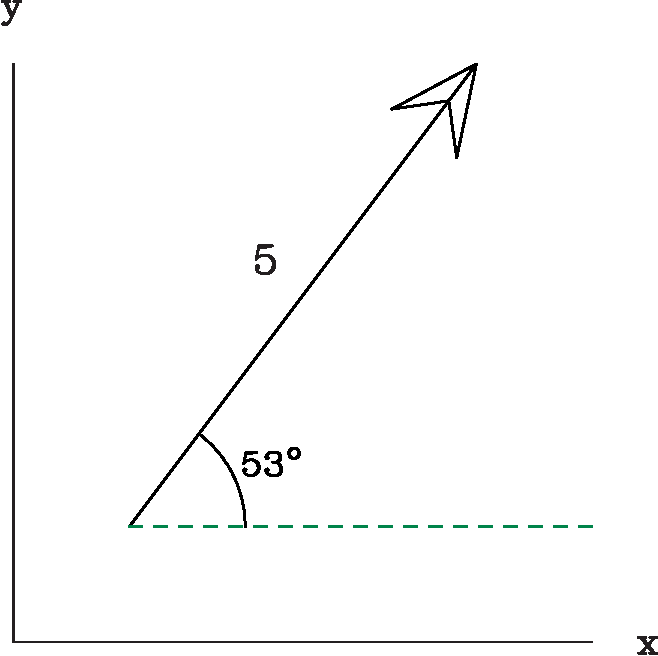
\includegraphics[width=0.7\textwidth]{vector-angle-crop.pdf}}
\Large
\centerline{Angle and direction}
\column{0.5\textwidth}
\centerline{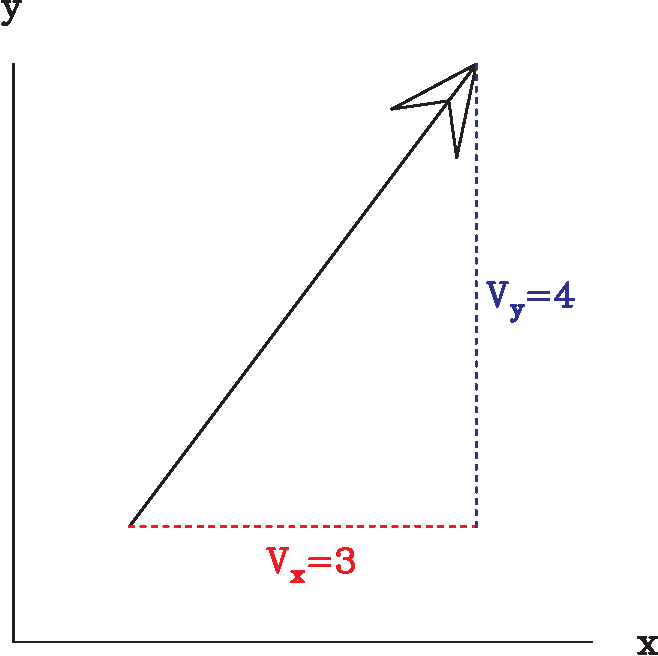
\includegraphics[width=0.7\textwidth]{vector-components-crop.pdf}}
\Large
\centerline{X and Y components}
\end{columns}
\bigskip
\bigskip
\Large
\centerline{How do we convert from one to the other?}
}

\frame{\frametitle{\textbf{From ``direction and magnitude'' to components}}
\centerline{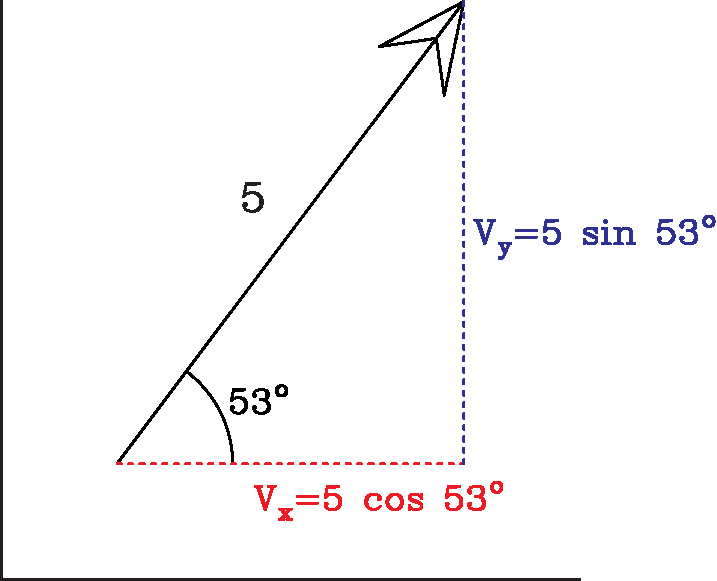
\includegraphics[width=0.6\textwidth]{vector-ang2comp-crop.pdf}}
}

\frame{\frametitle{\textbf{From components to direction and magnitude}}
\centerline{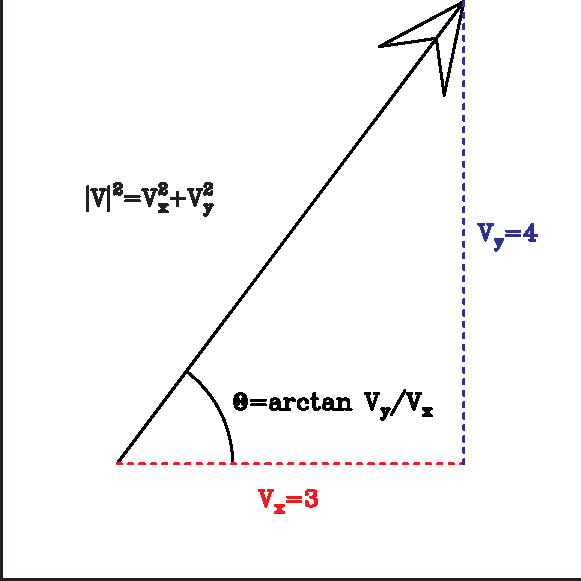
\includegraphics[width=0.6\textwidth]{vector-comp2ang-crop.pdf}}
}

\frame{\frametitle{\textbf{A warning!}}

\centerline{\Large{You cannot memorize ``$V \sin \theta$ is the $y$ component,}}  
\centerline{\Large{$V \cos \theta$ is the $x$ component''!}}
\bigskip
\bigskip
\centerline{\Large{This does {\it not} work in general; you have to actually draw the triangle.}}
}

\frame{\frametitle{\textbf{Adding vectors}}
We can also add vectors together by drawing them ``head to tail''. Here are two vectors:

\bigskip
\bigskip

\begin{columns}
\column{0.5\textwidth}
\centerline{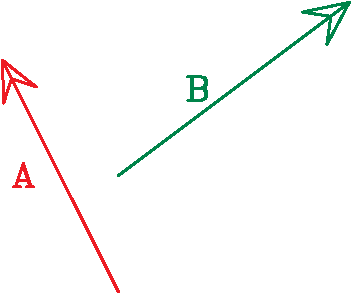
\includegraphics[width=0.6\textwidth]{vshow-crop.pdf}}
\column{0.5\textwidth}
\centerline{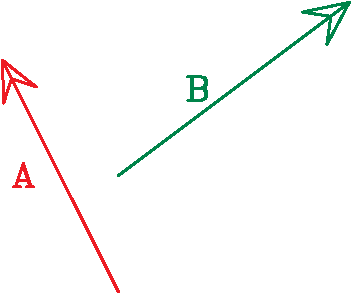
\includegraphics[width=0.6\textwidth]{vshow-crop.pdf}}
\end{columns}
}

\frame{\frametitle{\textbf{Adding vectors}}
\centerline{We can also add vectors together by drawing them ``head to tail''. Here are two vectors:}

\bigskip
\bigskip

\begin{columns}
\column{0.5\textwidth}
\centerline{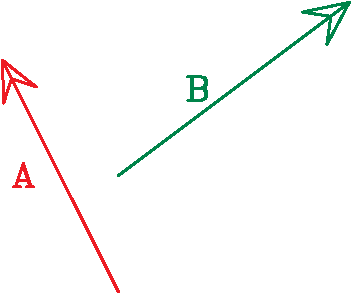
\includegraphics[width=0.6\textwidth]{vshow-crop.pdf}}
\column{0.5\textwidth}
\centerline{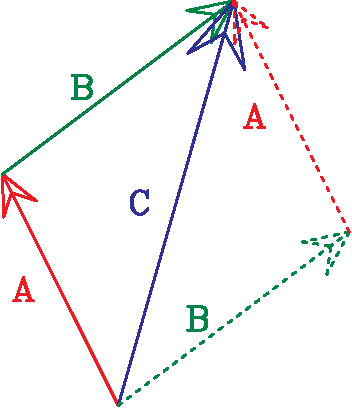
\includegraphics[width=0.6\textwidth]{vadd-crop.pdf}}
\end{columns}

\bigskip
\bigskip

\Large \centerline{$\color{Red}\vec A + \color{Green} \vec B = \color{Blue} \vec C$}

}

\frame{\frametitle{\textbf{Adding vectors: components}}
\centerline{\Large The component representation is much easier to work with!}

\Huge\centerline{$\color{Red}\vec A + \color{Green} \vec B = \color{Blue} \vec C \color{Black} \rightarrow {\color{Red} A_x + \color{Green} B_x = \color{Blue} C_x \choose \color{Red} A_y + \color{Green} B_y = \color{Blue} C_y}$}
}

\frame{\frametitle{\textbf{Adding vectors: components}}
\centerline{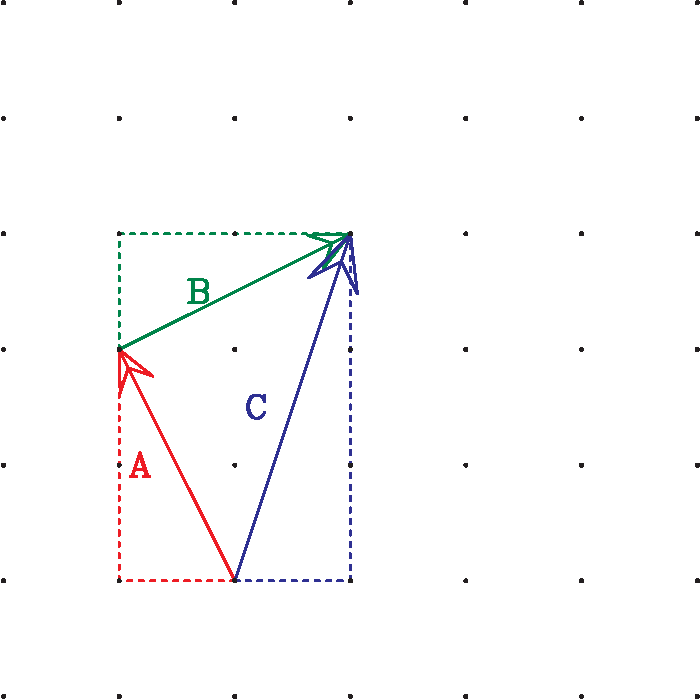
\includegraphics[width=0.4\textwidth]{vaddc-crop.pdf}}

\large
\bigskip

\centerline{To add two vectors, just add their components!}

\bigskip

\centerline{This is why it is almost always easiest to work in the component representation!}
}

\frame{\frametitle{\textbf{What does this do to our kinematics?}}
\large Acceleration, velocity, and position relationships are still the same; they just apply {\color{Red}independently} for each component.
\Large

\begin{align*}
\vec v(t) =&\, \vec at + \vec v_0 \\
\vec r(t) =&\, \frac{1}{2}\vec a t^2 + \vec v_0 t + \vec r_0
\end{align*}

\pause

\begin{align*}
\vec v_x(t) =&\, a_x t + v_{x,0} \\
\vec v_y(t) =& a_y t + v_{y,0} \\
\end{align*}
\pause
\begin{align*}
\vec x(t) =&\,  \frac{1}{2}  a_x t^2 + v_{x,0} t + x_0\\
\bigskip
\vec y(t) =&\, \frac{1}{2}  a_y t^2 + v_{y,0} t + y_0
\end{align*}
}

\frame{\frametitle{\textbf{Problem solving: 2D kinematics, constant acceleration}}
\Large
\begin{enumerate}
\item{1. If you have vectors in the ``angle and magnitude'' form, convert them to components}
\item{2. Write down the kinematics relations, separately for $x$ and $y$}
\begin{itemize}
\large
\item{Many terms will usually be zero}
\item{Freefall: $a_x = 0$, $a_y = -g$ (with conventional choice of axes)}
\end{itemize}
\item{3. Understand what instant in time you want to know about}
\item{4. Put in what you know; solve for what you don't (using substitution, if necessary)}
\item{5. Convert vectors into whatever format the problem asks for}
\end{enumerate}
}

\frame{\frametitle{\textbf{Sample problems}}
\centerline{\Large{A rock is thrown at $10 m/s$ at $30^\circ$ above the horizontal.}}

\bigskip
\bigskip

\begin{itemize}
\large
\item{How far from its starting point is it after 2 seconds?}
\pause
\item{How far does it travel?}
\pause
\item{How high does it go?}
\pause
\item{What will its speed be when it strikes the ground?}
\end{itemize}
}
\end{document}
